% chap2.tex
\part{프로그램 구성}
\label{part:ioref}

% ---------------------------------------------------------------------------- %
%                                  NEW SECTION                                 %
% ---------------------------------------------------------------------------- %

\chapter{프로그램 구조}
본 엔진은 핵심 python 모듈(pyGRsim)과 함께, Python(3.12)\cite{python312}, EnergyPlus(24-2-0)\cite{energyplus242}를 무설치로 포함하여, 어떤 환경에서든 단독으로 실행 가능하게 제작되었다(그림 \ref{fig:package_structure}). 사실 말이 엔진이지 그냥 python 모듈을 만든 것이니 그냥 EP랑 python 버전 맞춰주고 python 모듈만 별도로 다운받아서 밑에 설명서 읽고 사용하면 충분히 모종의 목적으로 사용 가능하다.

\begin{defaultfigure}
  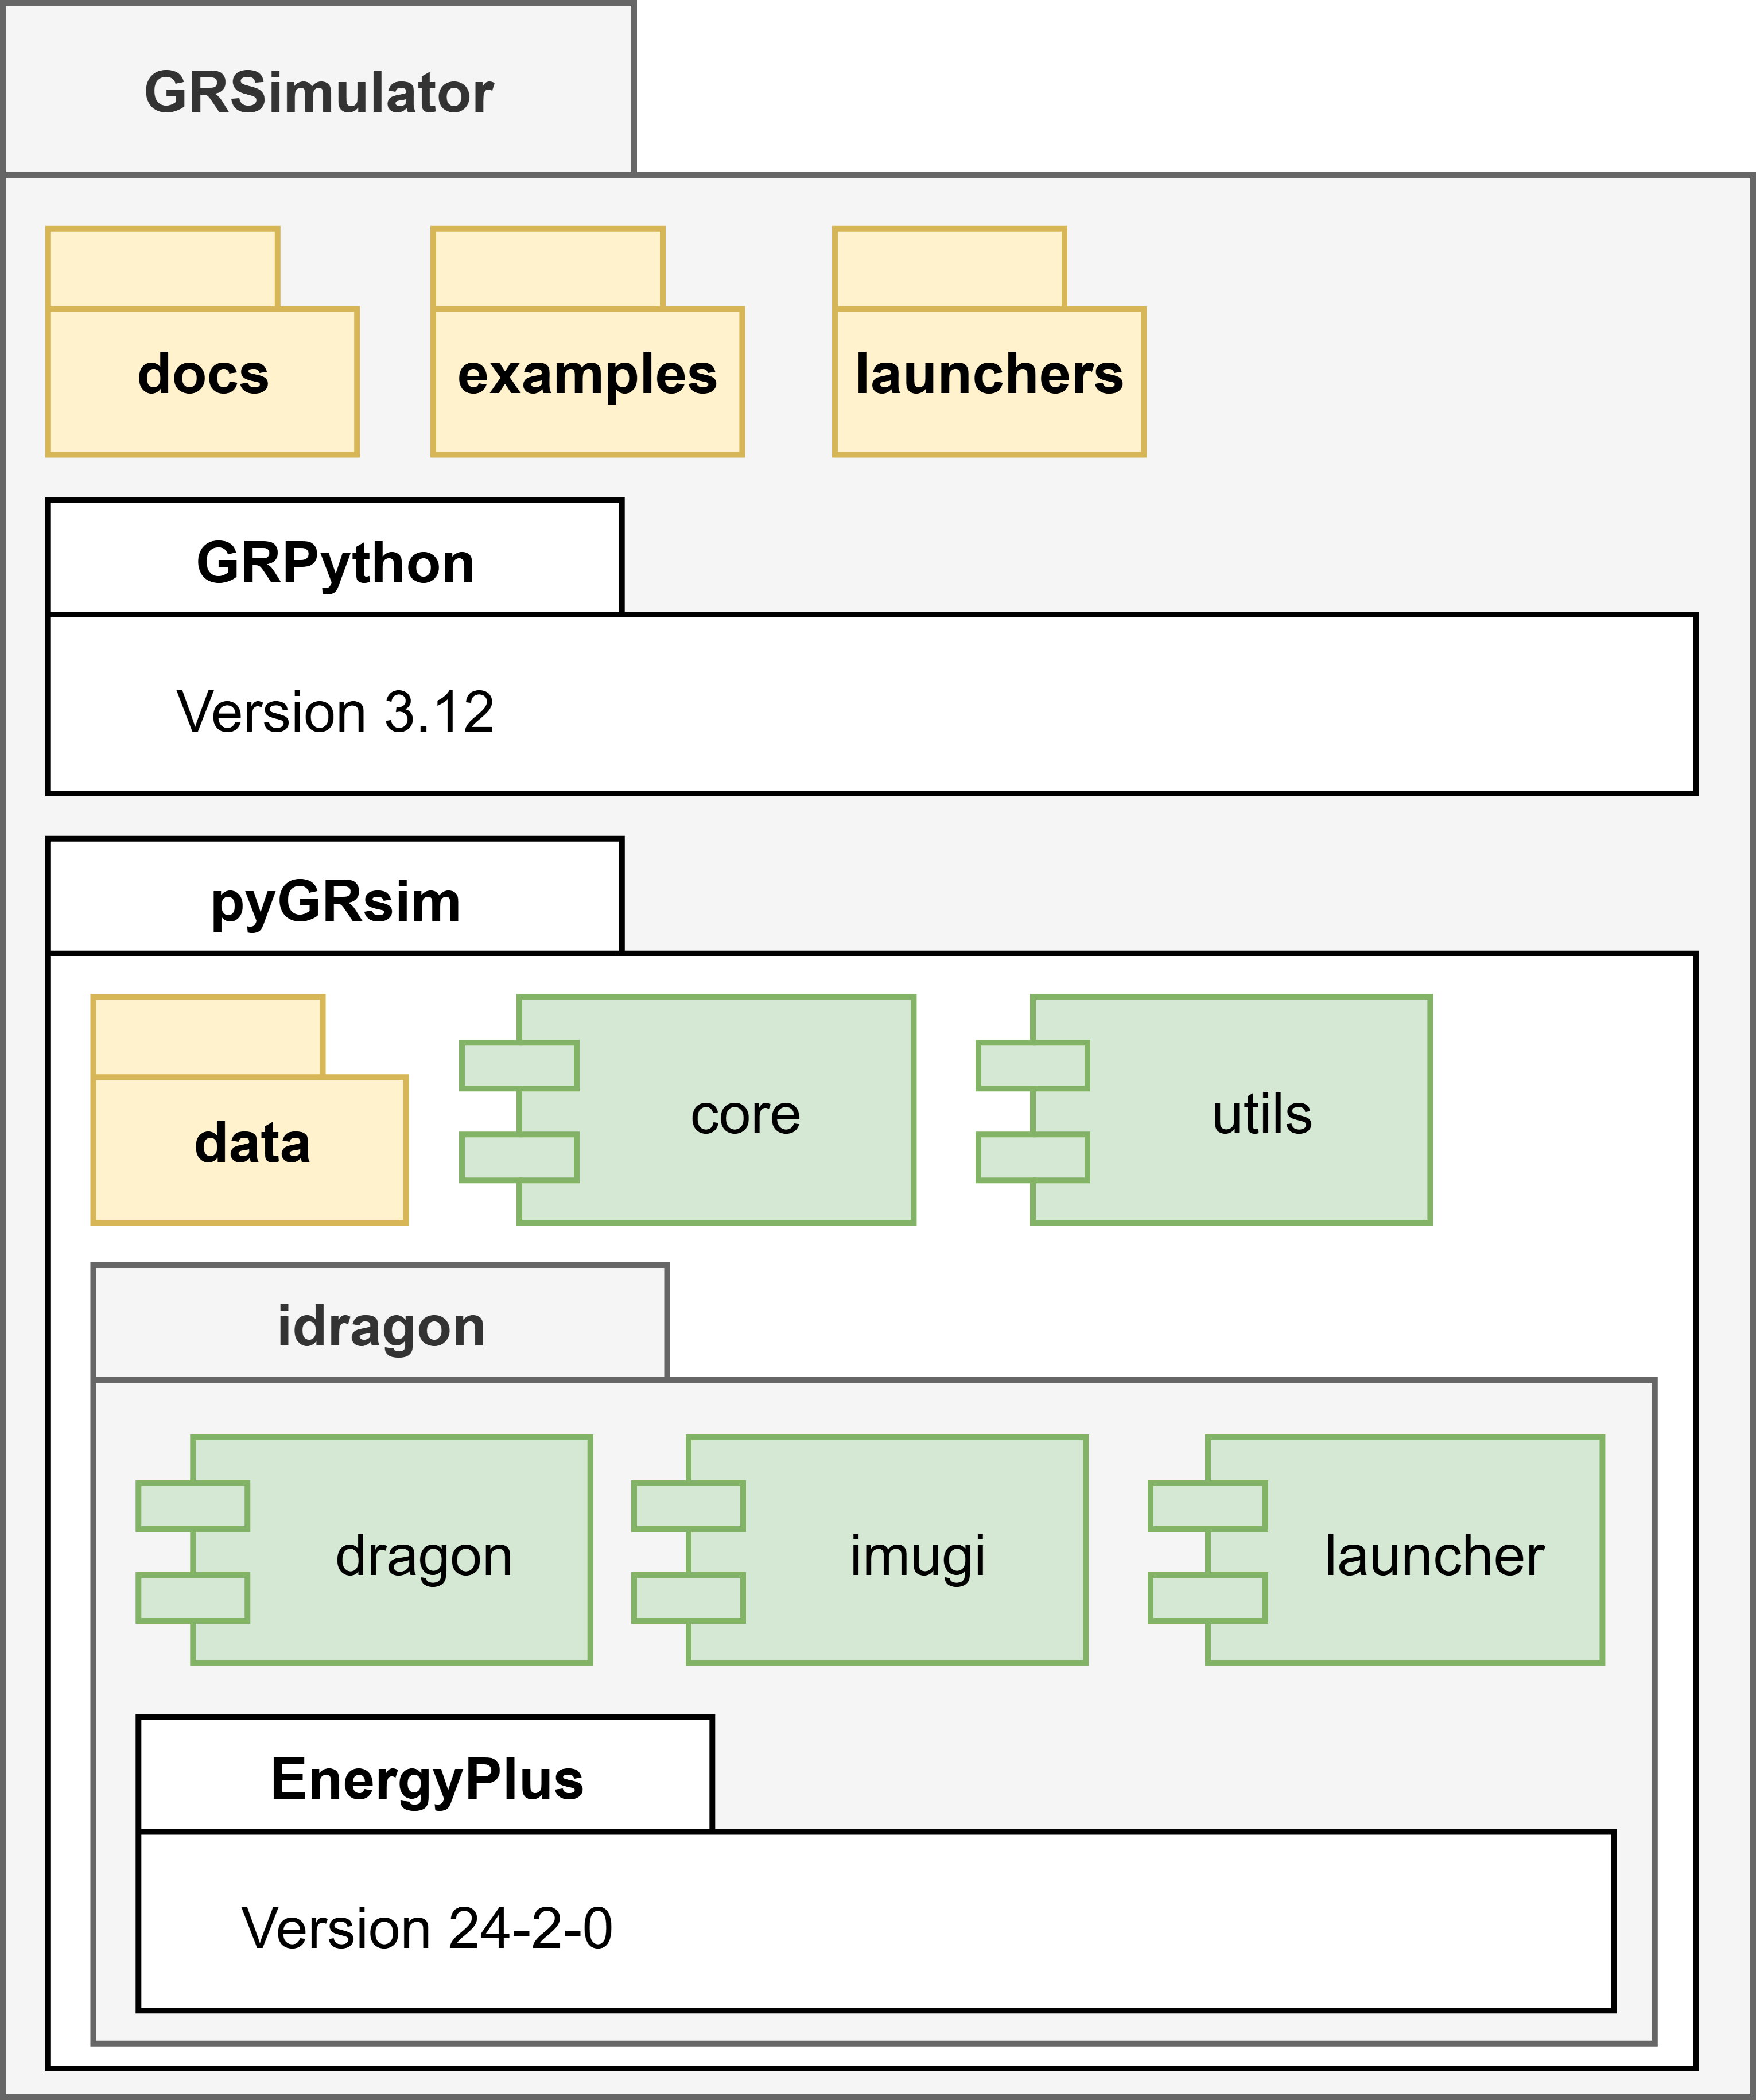
\includegraphics[scale=0.1]{package_structure.png}
  \caption{\simulator\ 프로그램 구조도}
  \label{fig:package_structure}
\end{defaultfigure}

이 프로그램이 하는 건 실질적으로 converting이다 (그림 \ref{fig:package_function}). 중간에 python이 껴있고, interface로 IO 처리한다.

\begin{defaultfigure}
  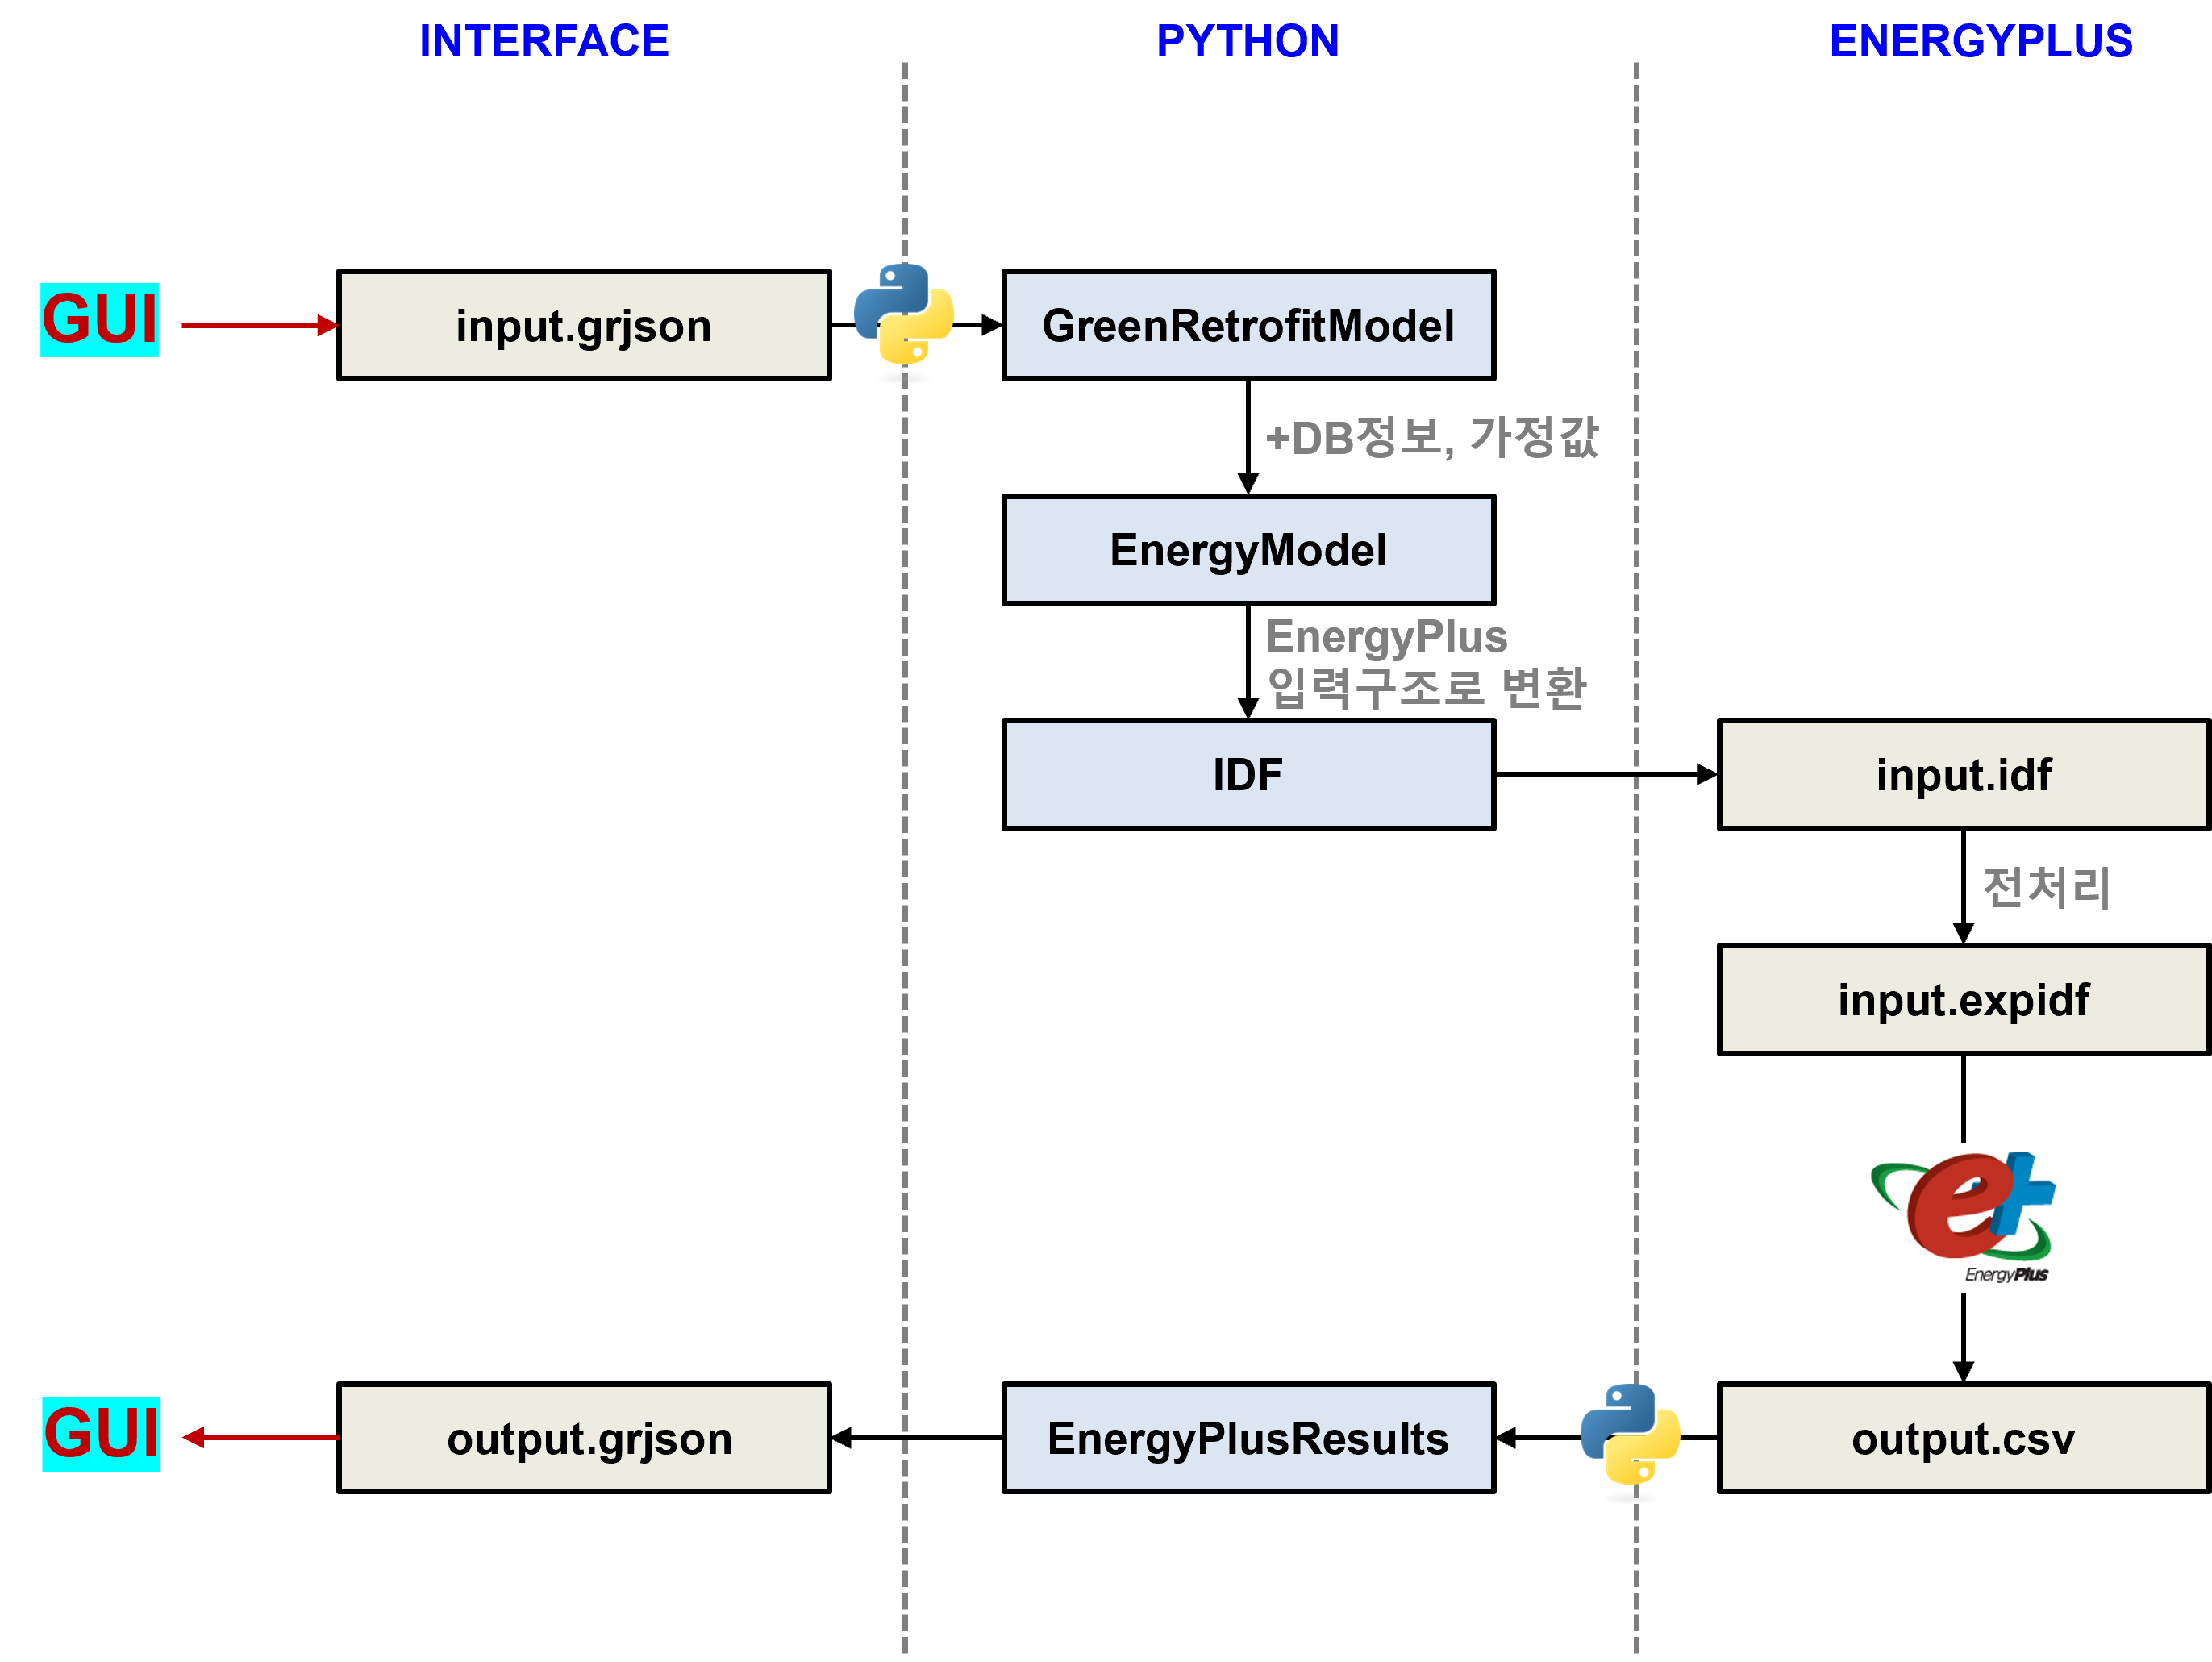
\includegraphics[width=\textwidth]{GRSimulator의 실체.png}
  \caption{\simulator\ 프로그램의 기능...이 무엇인지?}
  \label{fig:package_function}

  
\end{defaultfigure}

\section{Python 및 그 모듈}
Python 3.12를 쓴다. 3.11까지는 호환되는거같다. 그 아래로는 잘 모르겠다. \par
pandas랑 numpy 정도는 쓴다 얘네들도 각각 버전이 있다. 호환성은 체크 안해봤다.

% ---------------------------------------------------------------------------- %
%                                  NEW SECTION                                 %
% ---------------------------------------------------------------------------- %

\section{EnergyPlus}
EnergyPlus 24.2를 쓴다. 이건 상하위호환 둘 다 안되니까 설치하려면 정확하게 해야 한다. (사실 될 수도 있는데 굳이 체크 안해봐도 될 듯)\par
참고로 그냥 일반적으로 설치되는 경로인 C:/EnergyPlusV24-2-0에 깔려있으면 이 모듈이랑 같이 묶지 않아도 알아서 찾아서 돌릴 수 있다. EP찾는 순서는 아래와 같다.

\begin{enumerate}
  \item dragon 아래에 있는 EP 폴더
  \item C드라이브에 있는 기본 설치 폴더
  \item 그다음에 내가 그냥 새로 깔기
\end{enumerate}

원래는 자동으로 설치하는 옵션같은것도 고려하려고 했는데 배포 시점에 가능할지는 의문.

% ---------------------------------------------------------------------------- %
%                                  NEW SECTION                                 %
% ---------------------------------------------------------------------------- %

\section{예시파일 및 기타 문서}
도 준비되어있다.

설명 문서가 준비되어 있다.
\begin{itemize}
  \item 이 문서랑 별개로 PPT로 만든 사용자 매뉴얼이 제공된다.
  \item 이 문서는 개발자, 연구자용이다.
  \item 개발 과정을 담은 보고서는 어디에 공개되어있으니 별도로 참고 바람.
\end{itemize}

예시파일들도 준비되어있다. 표준입력과 출력을 n개 건물에 대하여 준비하였다.
(이 건물들을 어떻게 정의할 것인지, 건물명을 노출하지 않더라도 그 모델을 노출하는 것이 맞을지 논의가 필요할 듯)

\begin{itemize}
  \item grjson 예시도 준비되어있다.
  \item grexcel 예시도 준비되어있다.
  \item grresult 예시도 준비되어있다.
\end{itemize}


% ---------------------------------------------------------------------------- %
%                                  NEW SECTION                                 %
% ---------------------------------------------------------------------------- %

\section{보조 프로그램들}
도 만들어봤다.
bat파일로 만든거니까 실행할 때 조심하시고.. 서버 안꺼질 수도 있으니까 조심하시고... \textbackslash taskkill로 python 다 죽이는 것 권장한다. \par
go로 GUI를 simple하게 만들어서 배포??? ...는 좀 아닌 것 같긴 함. 내가 시간이 진짜 많으면 가능할지도? 할거면 그냥 JS로 하는 게 맞다 chart.js같은거 이식 못한다고 본다.

\subsection{grexcel 검토 launcher}
CHECK\_GREXCEL.bat 파일 실행하면 된다. 그럼 이런 창이 뜬다 (그림 \ref{fig:grjson_checker_capture}).
파일 선택누르고 check 누르면 좀 기다려야 한다. 다 되면 초록색으로 이렇게 뜬다.

\begin{defaultfigure}
  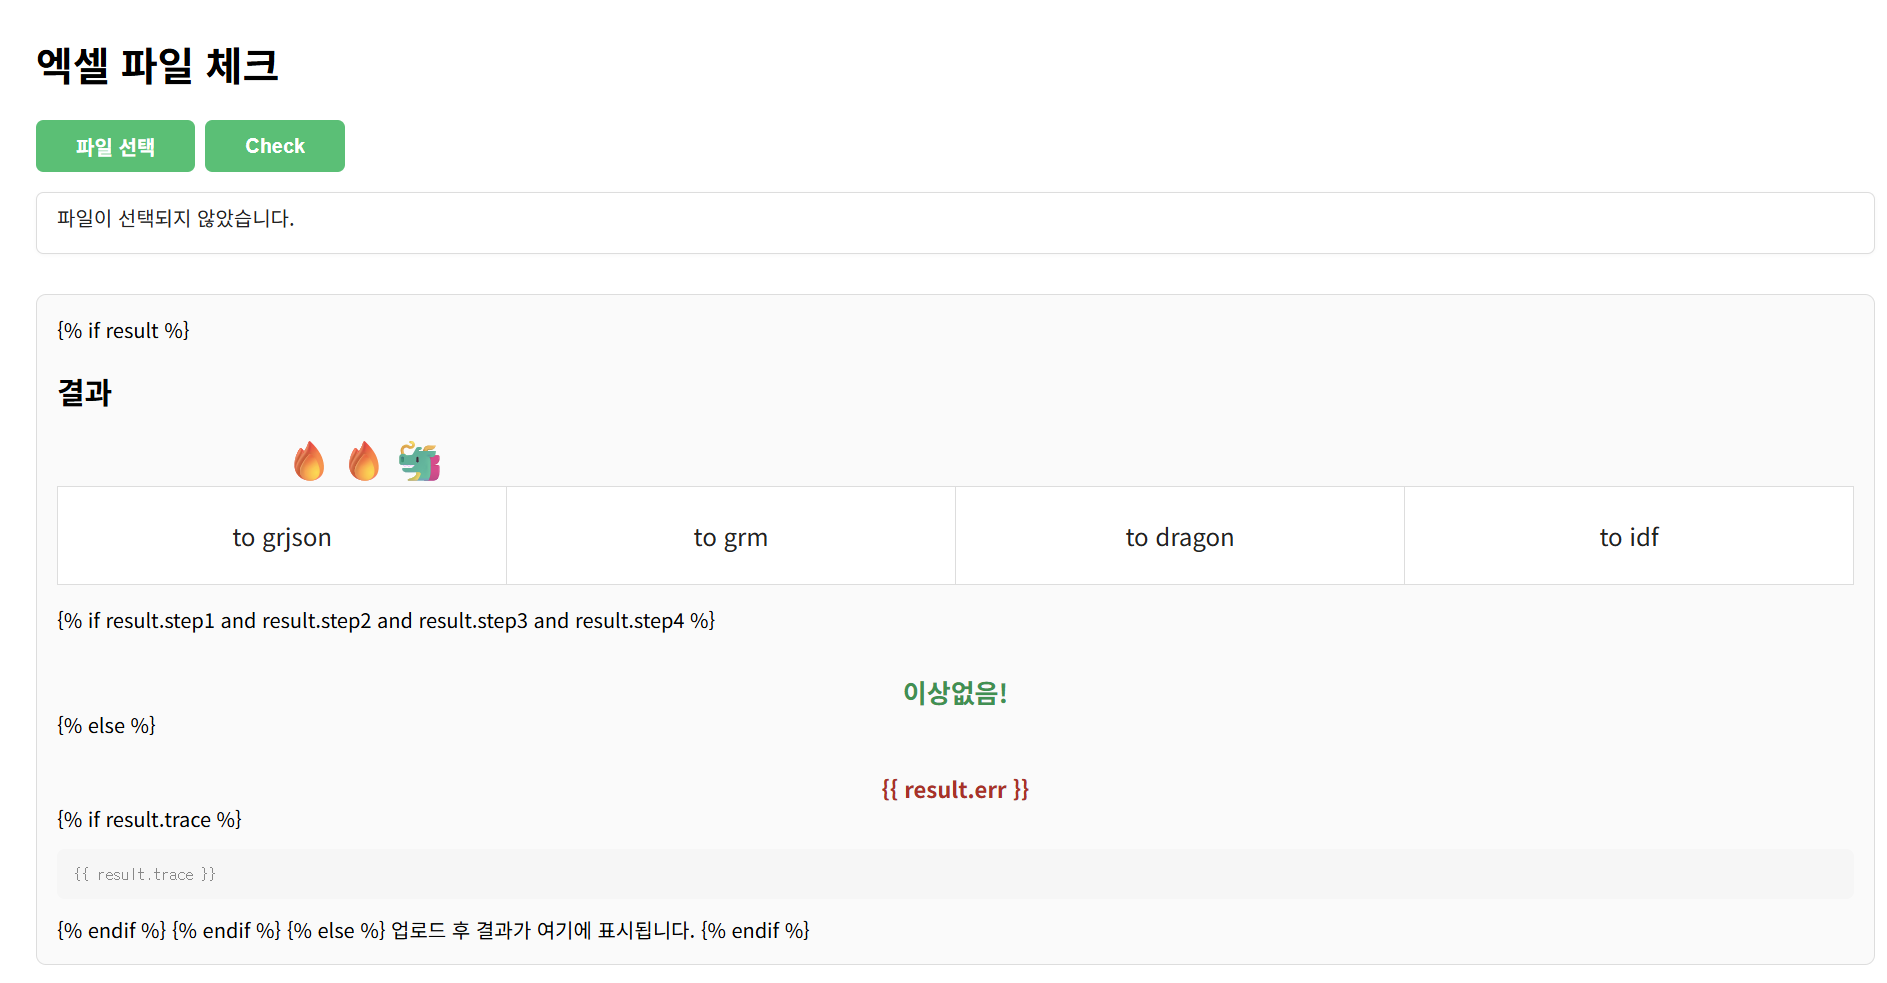
\includegraphics[width=\textwidth]{grexcel checker 캡처.png}
  \caption{grexcel checker 실행하면 나오는 페이지}
  \label{fig:grjson_checker_capture}
\end{defaultfigure}

\subsection{grexcel 실행 launcher}
RUN\_GREXCEL.bat 파일 실행하면 된다. 그럼 이런 창이 뜬다 (그림 \ref{fig:grjson_launcher_capture}).

\begin{defaultfigure}
  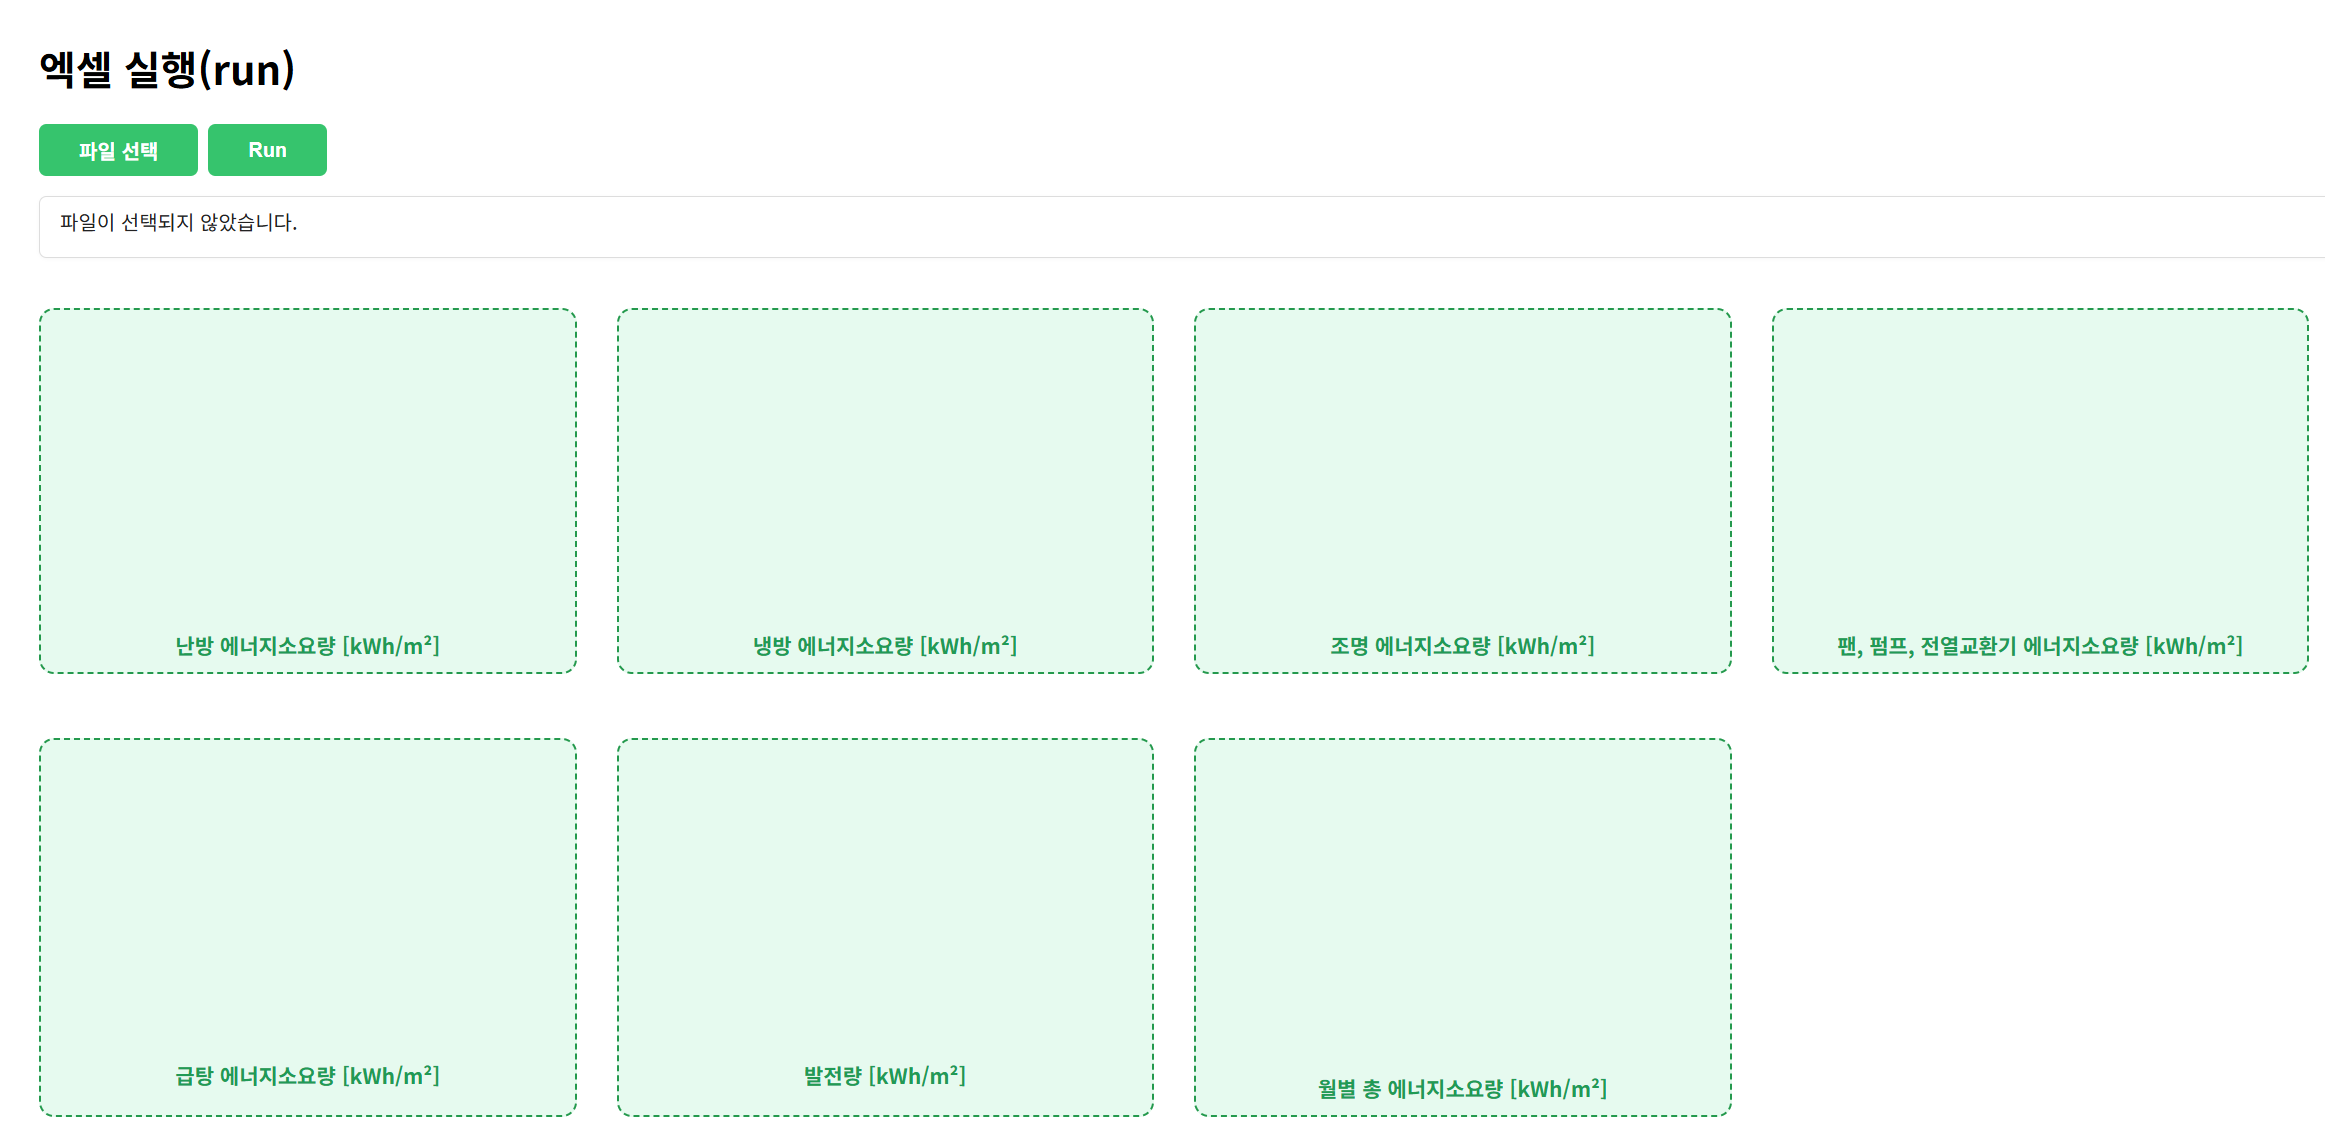
\includegraphics[width=\textwidth]{grexcel launcher 캡처.png}
  \caption{grexcel runner 실행하면 나오는 페이지 (시뮬레이션 전)}
  \label{fig:grjson_launcher_capture}
\end{defaultfigure}

파일 선택하고 run 누르면 좀 기다려야 한다. 다 되면 초록색으로 이렇게 (그림 \ref{fig:grjson_launcher_capture (result)}) 뜬다.

\begin{defaultfigure}
  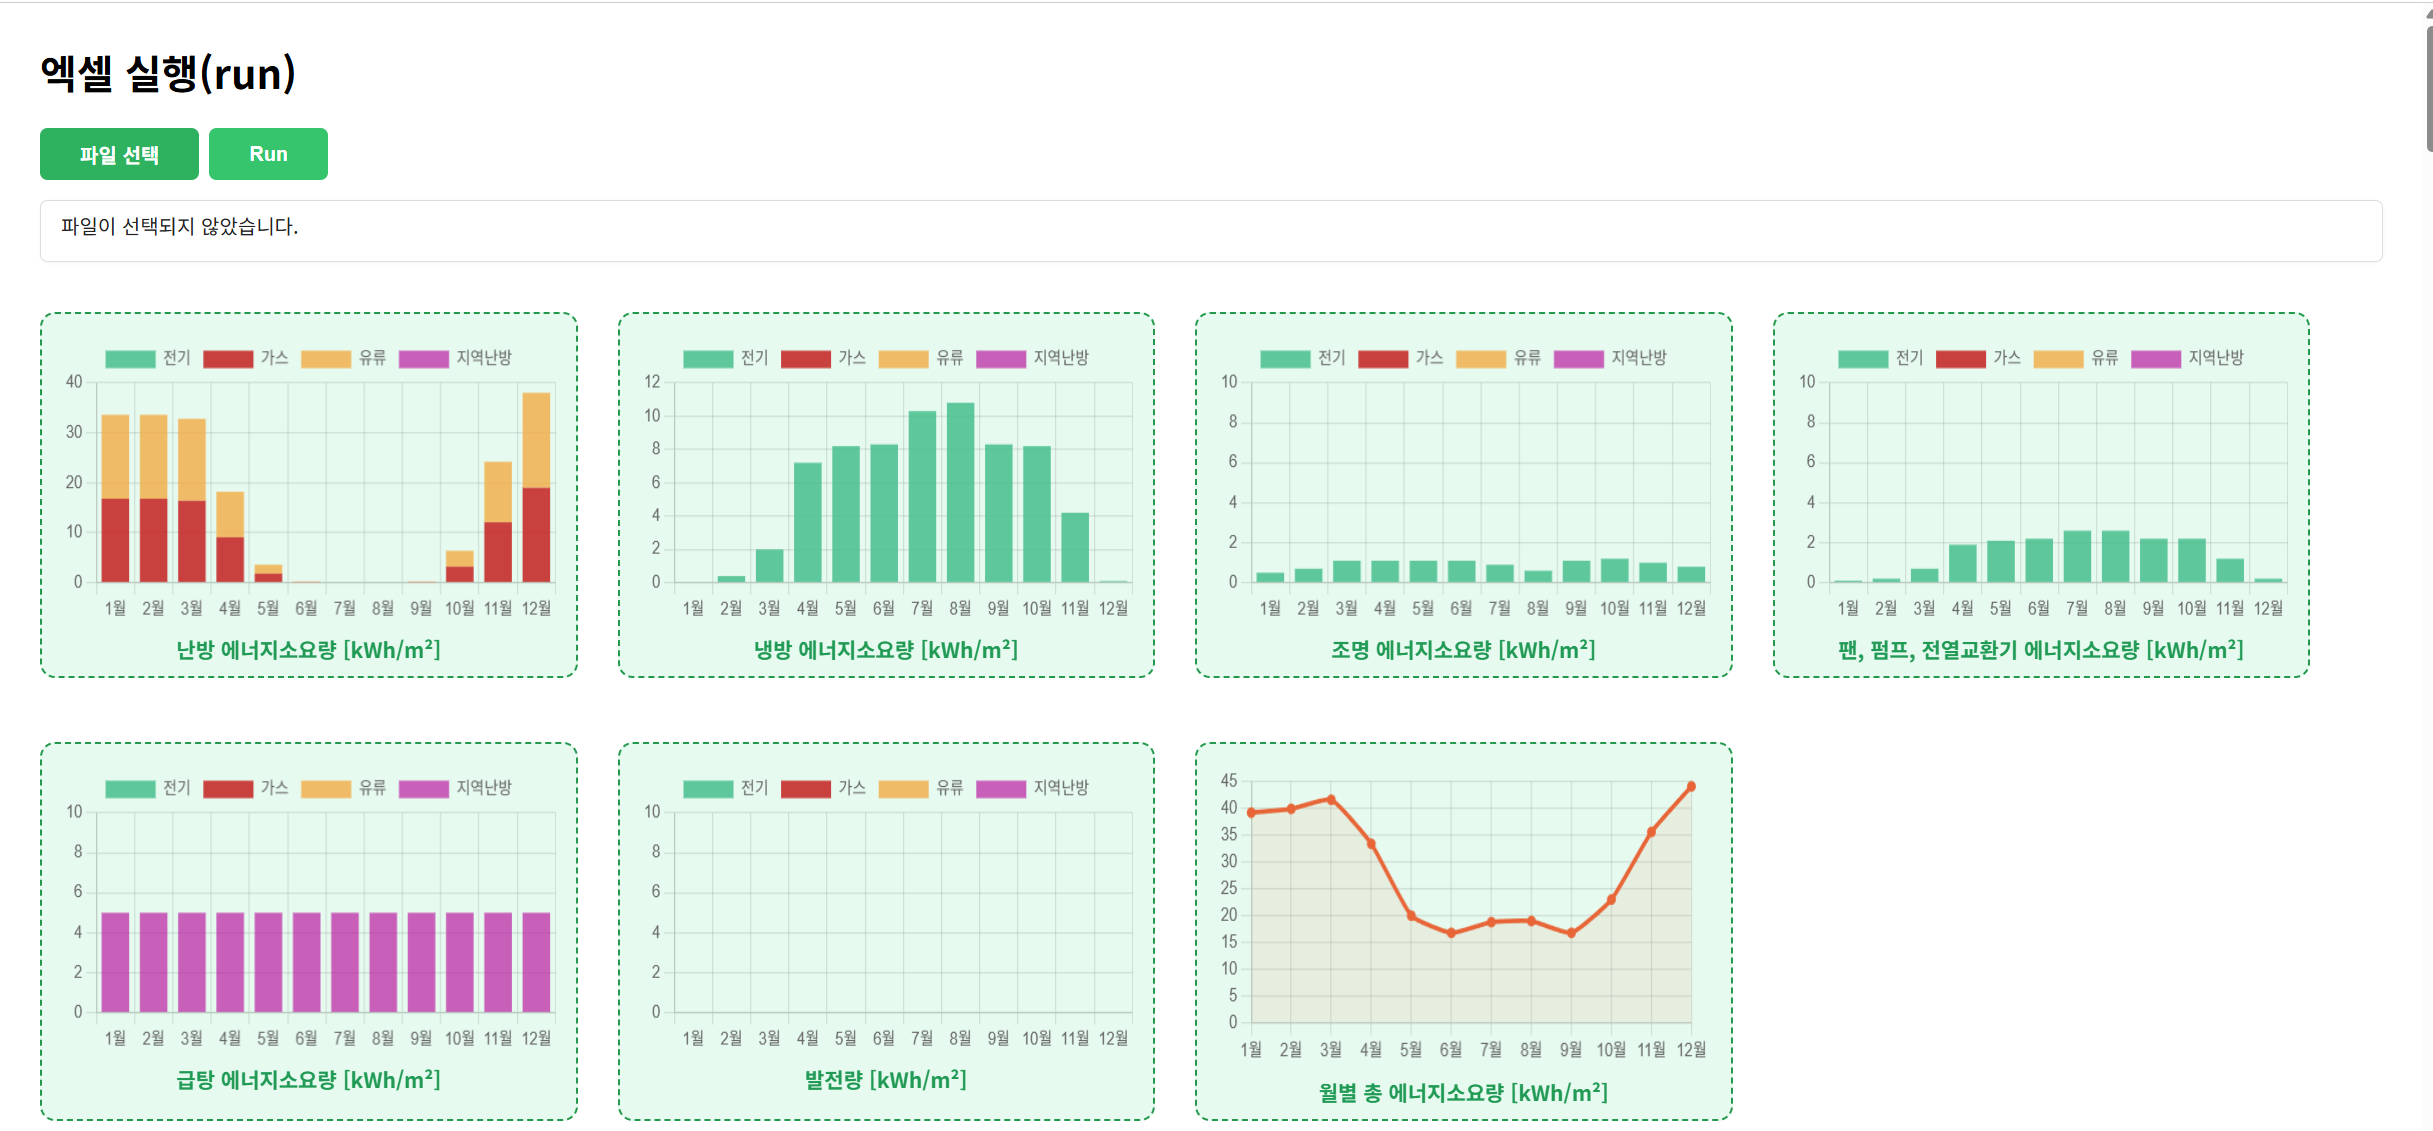
\includegraphics[width=\textwidth]{grexcel launcher 캡처 (결과).png}
  \caption{grexcel runner 실행하면 나오는 페이지 (시뮬레이션 후)}
  \label{fig:grjson_launcher_capture (result)}
\end{defaultfigure}

\subsection{grjson 실행 launcher}

이것도 하나 있어야 되나? launcher를 통합?

\subsection{grjson viewer}

zone간 연결관계 등 표시할 수 있는 viewer 하나 개발해두면 좋을 듯.

% ---------------------------------------------------------------------------- %
%                                  NEW SECTION                                 %
% ---------------------------------------------------------------------------- %
\chapter{입력 및 출력 파일 명세}



\section{\simulator의 데이터 구조}
본 엔진의 입력 데이터는 건물 데이터와,... 이다 (\ref{fig:grjson_structure}).

\begin{defaultfigure}
  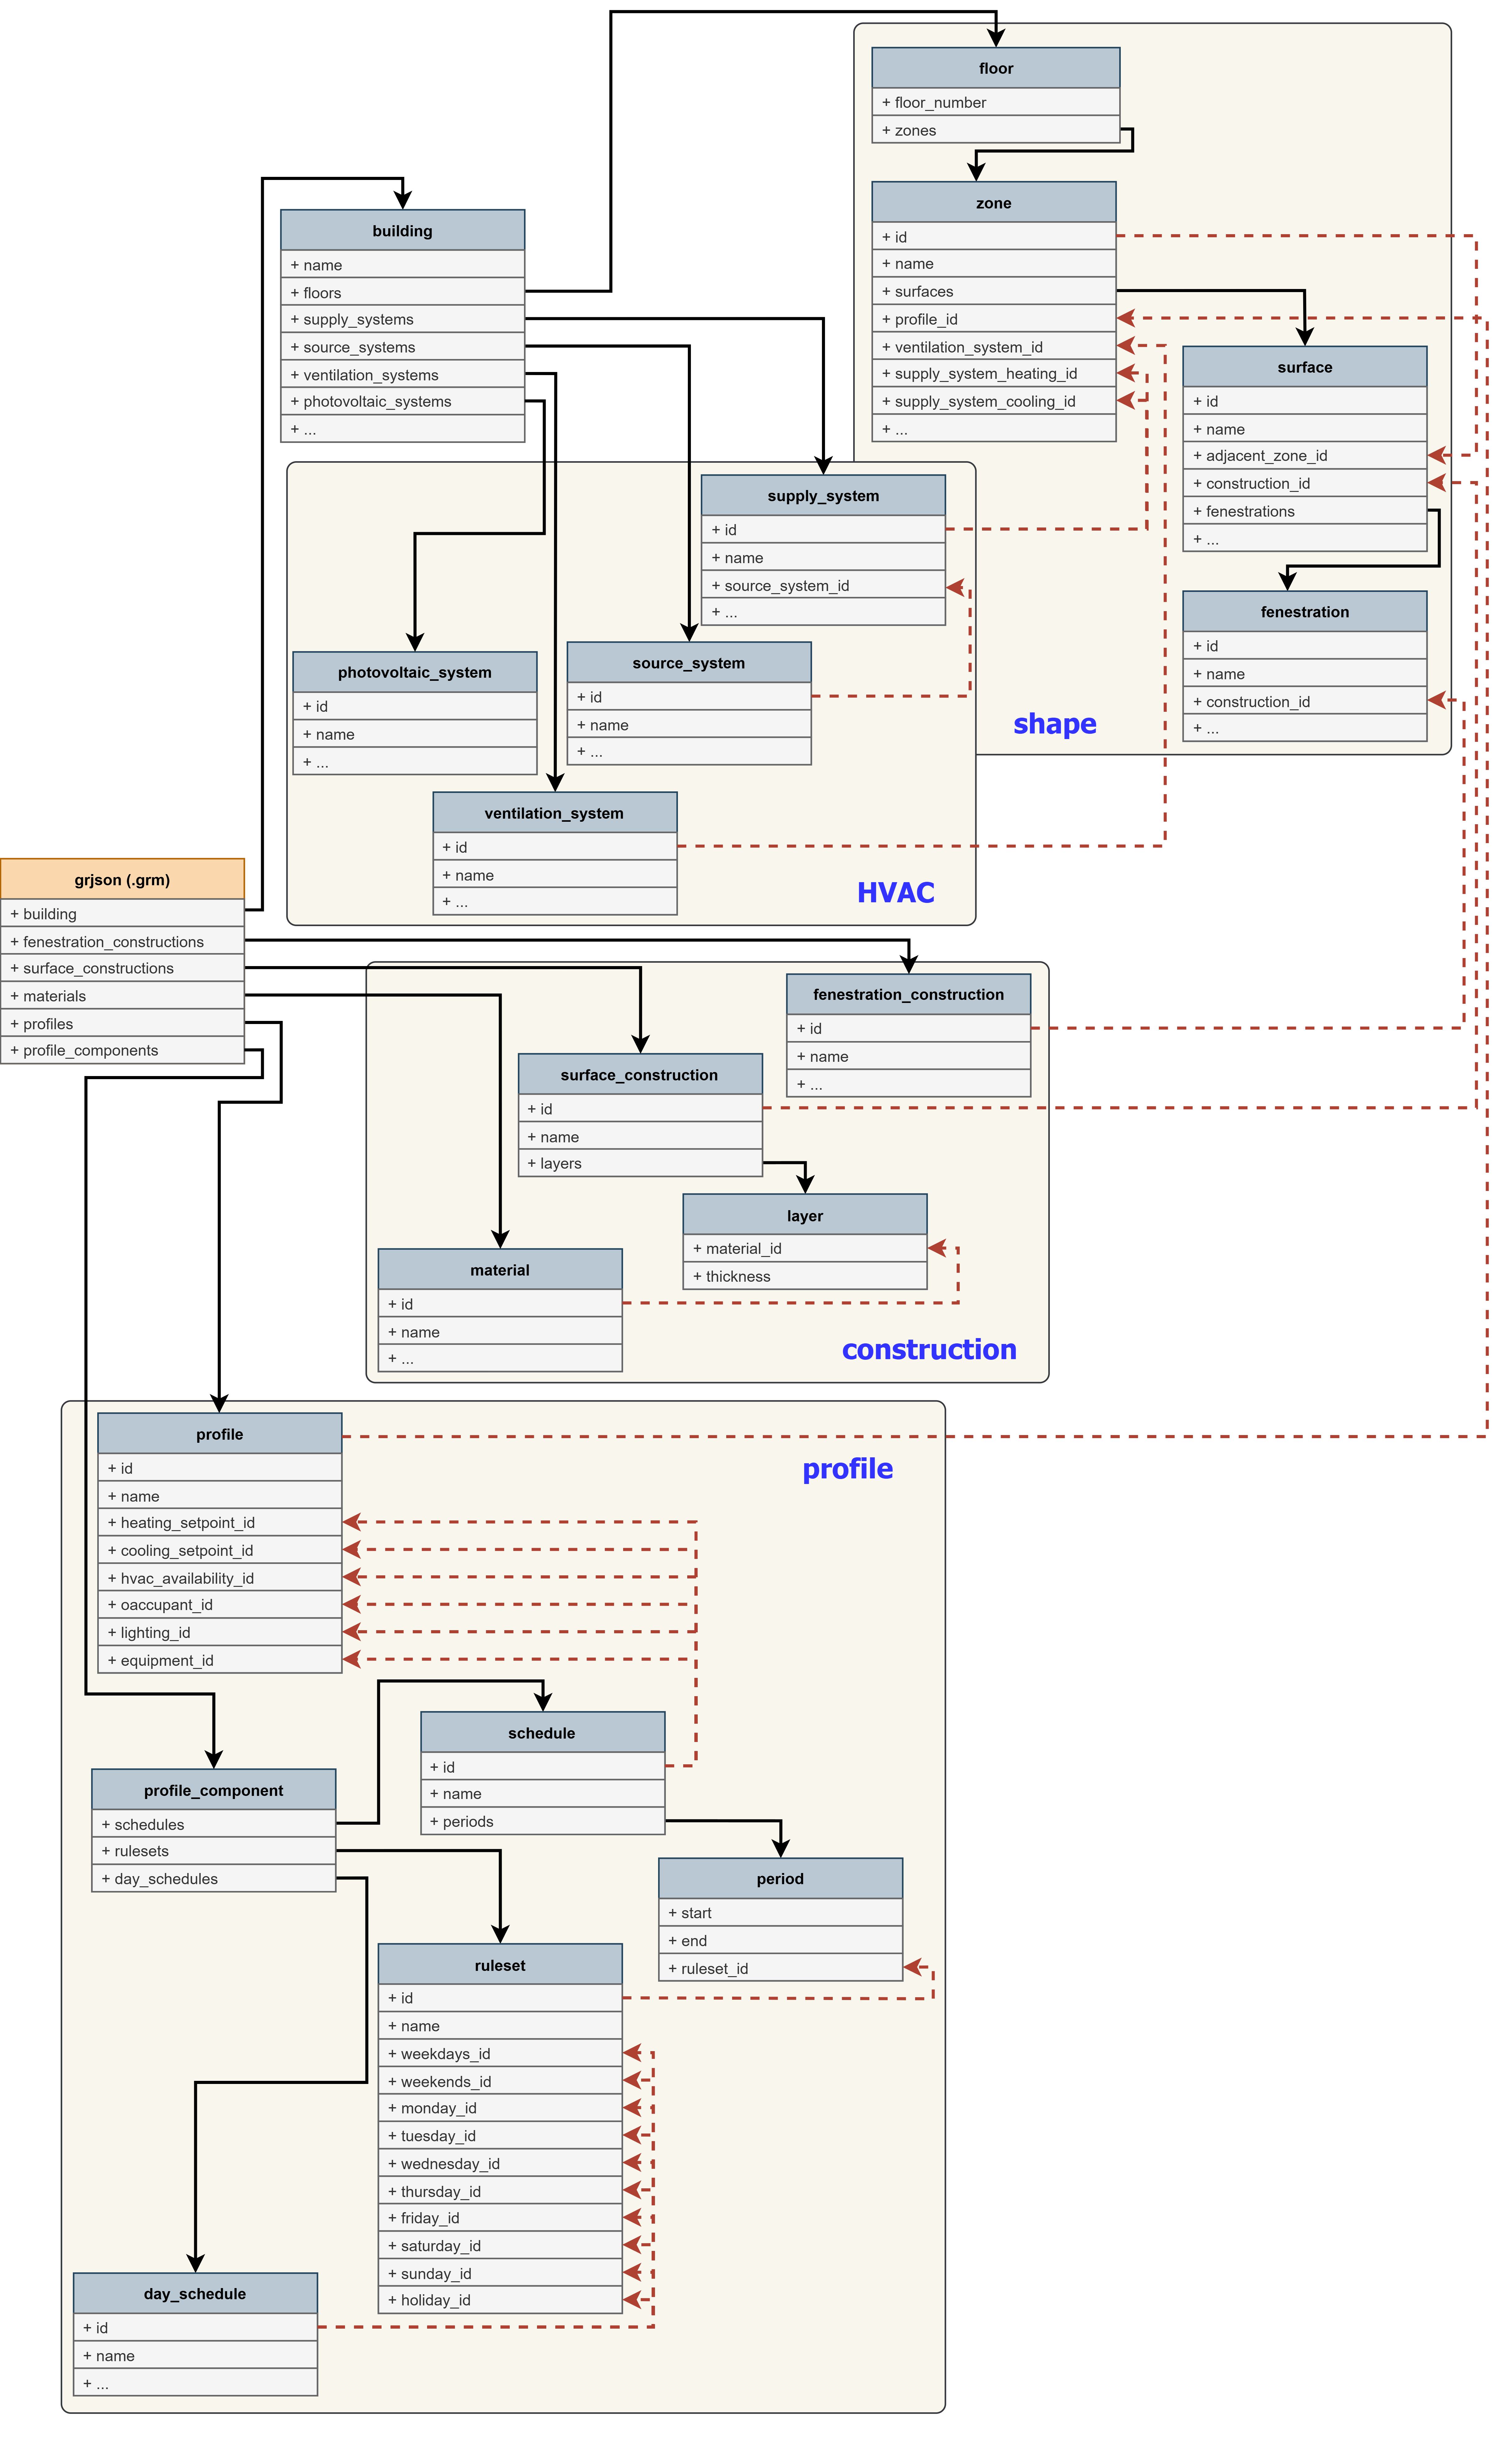
\includegraphics[height=0.99\textheight]{grjson_input_structure_v3.png}
  \caption{\simulator\ 입력변수 체계도}
  \label{fig:grjson_structure}
\end{defaultfigure}

% ---------------------------------------------------------------------------- %
%                                  NEW SECTION                                 %
% ---------------------------------------------------------------------------- %

\section{grjson 구조 (.grm 파일)}
\subsection{개발 규칙}
이 section은 향후 grjson을 수정하는 사람도 기억해야 하는 규칙임

\subsubsection{변수명}
\begin{itemize}
  \item 모든 변수명은 영문 소문자, 또는 밑줄(\_)로만 구성
  \item 복수 객체 list를 담는 변수명은 복수형 (e.g. “floors”), 단일 객체 dict, value를 담는 변수명은 단수형 (e.g. “name”)
  \begin{itemize}
    \item 복수 객체를 담는 하위 분류를 사용하는 객체는 상위 변수도 복수형 사용함\\
    (e.g. “profile\_components”)
    \item 길이가 정해져있거나 각 위치별 의미가 명시적으로 다른 경우는 예외\\
    (e.g. “vintage”: [1998,1,22])
  \end{itemize}
  \item 축약형 사용하지 않음 (e.g. supply\_sys → supply\_system, floor\_num → floor\_number)
  \item 약어 자체로 의미화 된 경우 사용: cop\_heating/cop\_cooling (coefficient of performance \_heating/cop\_cooling)
  \item 다른 class의 id를 참조하는 속성은 변수명 끝에 “\_id” 접미사 사용
\end{itemize}

\subsubsection{ID 기반 객체 참조}
grjson은 ID기반으로 객체 참조를 관리함.
\paragraph{사용가능한 문자} 모든 ID는 영문 대소문자, 숫자, 하이픈(-), 밑줄(\_)로만 구성, 숫자로 시작하지 않음
\paragraph{ID의 중복} 원칙적으로는 같은 class 내에서만 중복되지 않으면 문제없으나, 모든 class 간 중복되지 않는 것을 권장
\paragraph{권장} 서울대는 \verb|"${class구분자:4s}-0x${16진수index:06d}"| 형태로 임의생성중 (강제성 없음)

\subsubsection{기타 규칙}

\paragraph{속성의 명시 여부}
타 속성 값에 따라 불필요해지는 속성의 경우, 속성 자체를 작성하지 않음을 원칙으로 함. null값 출력해도 시뮬레이션에 문제 없음 → 본 규칙으로 export과정이 과하게 복잡해지는 경우 폐기 가능한 규칙임. e.g.) suface.type == “ceiling”이면 “azimuth” 속성 자체가 없음. 속성값을 없음으로 표현해야하는 경우 null로 표기. e.g.) 난방을 하지 않는 profile의 경우 heating\_setpoint 속성을 null로 표기

\paragraph{단위}
모든 속성값은 SI 기본단위 사용함 (m, J, W, kg 등)

\subsection{class별 명세}
\subsubsection{file}
건물 정보를 담고 있는 \hyperref[subsection:ioref:building]{building} 객체와 거기에 들어갈 reference들을 관리하는 얘네들 객체로 분류할 수 있음.

\subsubsection{building} \label{subsection:ioref:building}
빌딩은 건물 정보에 대한 최상위 정보임

\begin{table}[ht]
  \centering
  \begin{tabularx}{\textwidth}{l c c c c}
    \toprule
    변수명 & 타입  & 필수여부 & 조건(필요시) & 값 조건?\\ \midrule
    name & string & 필수 & & 건물 이름임 \\
    north\_axis & numeric & 필수 & & 0 이상 360 미만 \\
    address & string & 필수 & & 똑바로 써야함. \\ \bottomrule
  \end{tabularx}
\end{table}

\paragraph{name} 이름이다.
\paragraph{north\_axis} 북쪽 바라보는 그거다. 도면에서 나침반이 반시계 방향으로 $\theta$만큼 돌아가있음"에서 $\theta$를 입력 (?) 도면상 나침반의 방향을 반시계방향을 +로 해서 입력? 
\begin{defaultfigure}
  \centering
  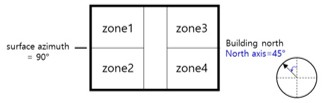
\includegraphics{north_axis 설명.jpg}     % 상대 경로 또는 절대 경로
  \caption{Building:north\_axis의 기준}
  \label{fig:example}
\end{defaultfigure}

\paragraph{address} 주소다. 이거 아래 예시처럼 시,군,구로 끝나야 한다.

\subsubsection{floor}
층구분이다.
\subsubsection{zone}
존이다.
\subsubsection{surface}
면이다.
\subsubsection{fenestration}
개구부다.
\subsubsection{supply\_system}
공급설비다.
\subsubsection{source\_system}
생산설비다.

\subsection{예시}
\subsubsection{AR모드, 모든 정보를 아는 경우}

모든 정보를 알면 아래 체계로 입력할 수 있다.

\subsubsection{AR모드, 벽체 속성 등 모르는 경우}

벽체 속성 등 모르는 경우엔 아래와 같이 비워둘 수 있다.

\subsubsection{OR모드}

아래는 스케줄도 직접 입력하는 예시이다. \par

code 구문에 한글 들어가있으면 컴파일 어려움 해결 필요

% ---------------------------------------------------------------------------- %
%                                  NEW SECTION                                 %
% ---------------------------------------------------------------------------- %

\section{grexcel 구조 (.xlsx 파일)}
\subsection{개발규칙}
얘는 사용자에게 제일 친화적으로 다가가는 게 목적임. 하나의 GUI를 표방한 것임. \par
단위도 사용자에게 편한 단위 쓴다. grjson이랑 다르게 두께는 mm쓰고 용량은 kW (맞나?) 쓴다.

\subsection{sheet별 명세}
\subsubsection{첫번째가 건물인가?}
아마도
\subsubsection{두번째가 실인가?}
그럴듯
\subsubsection{세번째부터 잘 모르나?}
그렇다.
\subsection{예시}
캡처
\subsection{grexcel을 grjson으로 변환하는 과정}

% ---------------------------------------------------------------------------- %
%                                  NEW SECTION                                 %
% ---------------------------------------------------------------------------- %

\section{grresult 구조 (.grr 파일)}
\subsection{class별 명세}
\subsubsection{입력정보 및 계산 방식 관련}
\paragraph{building} 건물 면적 등등 정보 포함함
\paragraph{constants} 계산에 사용된 상수값들 명시하는 것임. 이 값들의 출처는 n장 m절 참고바람.

\subsubsection{원시데이터 관련}
참고로 원시데이터는 다 면적당임 (확인필).
\paragraph{site\_uses} 건물에서 쓰는거 월별로 원별로 용도별로. 이런식으로 구성되어있음.
\paragraph{source\_uses} 1차에너지에 해당하는 것.
\paragraph{co2} CO2 배출량
\paragraph{cost} 비용. 여기까지 다 site\_uses에다가 곱해서 얻어지는 것임

\subsubsection{요약데이터 관련}
\paragraph{summary\_per\_area} 다 합한 것.
\paragraph{summary\_gross} 에 면적을 곱한 것. 비용 관련된 부분은 얘를 보는 게 맞을 듯.

\subsection{예시}

아래는 결과 파일 예시이다.

\subsection{다른 도구와의 관계}
\subsubsection{EnergyPlus(IDFEditor, DesignBuilder, ...)}
이걸 좀 더 사용자 친화적으로 바꾼 개념임. 형상은 이렇게 이해하면 되고 설비는 이렇게 이해해야 함. EP 설비할 때는 이런걸 이렇게 신경썼을텐데 이 툴을 쓸 때는 이런식으로 접근하면 대응되게 할 수 있음.

\subsubsection{ECO2}
입력체계는 거의 비슷하다. 원래 하던대로 하면 된다. 단 형상쪽은 좀 주의해야 할 것임. \par
결과도 비슷한데 환기쪽만 조심하면 됨. ECO2에서 환기는 환기침기부하지만 우리는 그런거 없음. 환기침기부하생기면 냉난방으로 처리하는 거니까 냉난방에 묶여있음. 써큘레이션이라고 팬 펌프 전열교환기만 따로 뽑았음.



% ---------------------------------------------------------------------------- %
%                                  NEW SECTION                                 %
% ---------------------------------------------------------------------------- %

\chapter{실행}

\section{요구 환경}
위에서 설명할것같은데 삭제해도 될지도? 위에서 언급안하는게 맞을지도 EP 설치할 수 있는 위치라던지 등등

% ---------------------------------------------------------------------------- %
%                                  NEW SECTION                                 %
% ---------------------------------------------------------------------------- %

\section{api}
\subsection{python 모듈의 실행 구조}
python -m 모듈이름 으로 시작하는거다. 우리 모듈도 똑같음 그걸 기대하고 만든것임 \_\_main\_\_.py가 진입점임.

\subsection{api 개발 원칙}
원칙까지는 없을듯.

\subsection{주요 api}

\subsubsection{run: grjson 또는 grexcel 실행}
호출하면 실행하는 것임 인자는 -i 또는 --input, -o 또는 --output 등 있음. 예시는 아래 코드 참고
\begin{tcolorbox}[colback=gray!10, colframe=gray!80, boxrule=0.5pt, left=1em, right=1em]
GRPython/python.exe -m pyGRsim run -i ...path\_to\_input/my\_grjson.grm
\end{tcolorbox}

\subsubsection{DB: DB값 조회}
호출하면 DB 조회하는 것임. DB 이름이랑 key를 보내면 됨. 예시는 아래 코드 참고.

\begin{tcolorbox}[colback=gray!10, colframe=gray!80, boxrule=0.5pt, left=1em, right=1em]
GRPython/python.exe -m pyGRsim run -i ...path\_to\_input/my\_grjson.grm
\end{tcolorbox}

참고로 surface construction이랑 fenestration construction은 \&로 묶은 key를 보내면 법규기준을 return하고 있음. \&로 묶을 수 있는 아이템들은 아래 참고 바람.